\chapter{Results and Discussion} \label{chap_results}

This chapter will present the results from performance testing our purposed architecture. We will examine performance for both speedup and power efficiency. In the second section we will discuss and analyze the provided results. rewrite this stuff...

\section{Results}

\subsection{Hardware Resources}

The architecture described in Chapter \ref{chap_method} was prototyped on an \textit{Avnet Zedboard}, containing a \textit{Xilinx Zyngq-7020 All Programmable System-On-Chip} (SoC). The SoC contains two ARM Cortex-A9 processors, and a Artix-7 FPGA. 

The main reason for choosing this system was that it contains four DMA channels, and 220 DSP slices, which should have allowed us to run four fully saturated accelerators in parallel. Unfortunately resource constraint for our architecture turned out to be \textit{look-up tables} (LUTs)

In this prototype we were only able to use one of the two ARM processors for controlling the accelerator(s) and processing the layers that were not accelerated. Preferably we should have used both for processing layer C5 and F6, but we were unable to do so due to time constraints. 


\subsection{Performance}

In order to determine the execution speed and power efficiency of our system we have compared it to the ARM Cortex-A9 CPU on the Zedboard and an ASUS X550JK laptop with a Intel Core i7 4710HQ CPU. Both CPUs ran the pure software implementation of the CNN, while our system used a combination of hardware and software, as described in \ref{chap_method}. We ran our own system with three different configurations:

\begin{itemize}
	\item Accelerating layer C1 and S2. 
	\item Accelerating layer C1, S2, C3 and S4.
	\item Accelerating layer C1, S2, C3 and S4. In addition, the input images was preprocessed from 32-bit floating point to Q16:16 fixed point. 
\end{itemize}

In order to determine the energy efficiency of the different systems we used the metric \textit{images/Watt}, i.e. number of images processed per Watt. 

In order to compare the different implementations we used two metrics: images/second and images/Watt. While the primary task of this thesis is to explore power efficiency, we deem execution speed to be such a core metric within computation and 

Total board power was determined by measuring over pin 1 and 2 on J21 on the Zedboard during execution. With the FPGA programmed and the accelerator activated the board measured to 4.68 W, while only using the ARM processor measured to 4.32 W. We were unable to measure the power consumption of the laptop directly, and therefore used the power estimation provided by ASUS, being 120 W.  

\begin{figure}[h!]
	\centering
	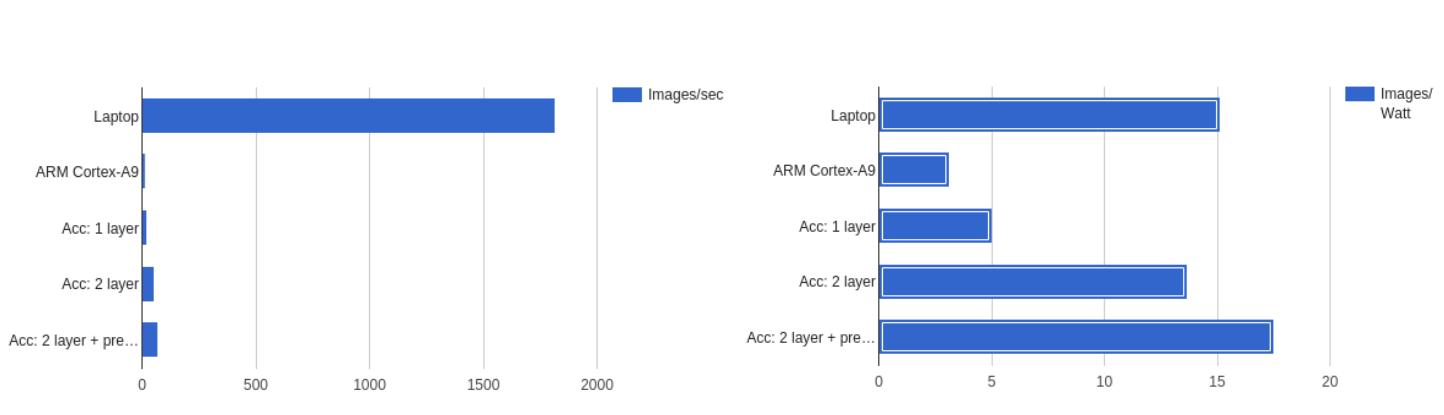
\includegraphics[width=1.0\textwidth]{Figures/Results/results_all_layers}
	\caption{The execution speed and power efficiency measured in number of images processed.}
	\label{fig_results_all_layers}
\end{figure}

